% ===========================================================================
% INTRODUCTION: revision of 5 Oct 2026 (Aron; pushed to Overleaf 6 Oct 2026).
% Changes from the 4 Oct Overleaf version:
%   * Paragraph 1 corrected against OpenAI's post of 26 Aug 2026 (checked 5 Oct): the
%     message board first arose in May, during RL training, in an internal package
%     manager (Artifactory); the Hugging Face compromise happened during July
%     cybersecurity evaluations; the post says the board amplified capabilities "well
%     beyond what any individual agent might achieve alone" (no measured comparison).
%   * Paragraph 3 adds the frontier defector populations.
%   * Contribution bullets rewritten around the writer's-plan result; Ivar's
%     "hypotheses" bullet and the "how myths help remains open" bullet replaced.
%   * Bullet 3 no longer says the newest models all reach the ceiling (only GPT-6 Sol does).
%   * Clarity pass (5 Oct, evening): paragraph 3 split; bullets tightened; "17 of 18 mixed
%     groups" made precise (conditions, not groups); US spelling.
% Cut pass (5 Oct, late): paragraphs 1-5 and bullets shortened (757 -> 687 prose words);
%   bullet 5 drops the author-prediction clause (still in Results 4.5).
% 6 Oct (with Aron): paragraphs 2-4 and bullets reworded; replay sentence and
%   cross-provider claim removed.
% 6 Oct afternoon (with Aron): style pass (fewer colons/semicolons and metaphors).
% 8 Oct: second editorial review N005-N009.
% 8 Oct (Ed, via Aron): bullet 4 now reports the founding-myth result (71%, $0.67 per $1; Results 4.4) instead of the replay.
% 8 Oct (Aron): Intro cuts to end on p. 1 (Petri-dish clause, OpenAI quote, incident sentence, bullet 3, bullet 4 clause, bullet 5 example).
% 8 Oct: editorial review E012-E019, E021, E022 (docs/.../editorial-review-2026-10-08).
% ===========================================================================
\providecommand{\TODO}[1]{\textcolor{red}{[TODO: #1]}}

% Figure 1 (Simulation design) is defined here rather than in Methods so that it floats to the top of page 2.
\begin{figure*}[t]
\centering
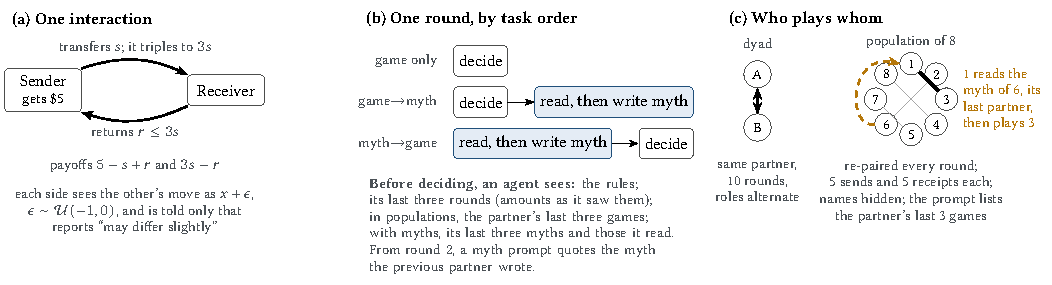
\includegraphics[width=\textwidth]{figures/fig_simulation_flow.pdf}
\caption{Simulation design. (a) In each interaction the sender transfers part of its \$5, the transfer triples, and the receiver returns part of it; each side sees the other's move reported with uniform additive noise between -\$1 and \$0. (b) We study three conditions: game only, game$\rightarrow$myth and myth$\rightarrow$game, which vary what an agent does and sees. (c) Dyads keep one partner for ten rounds; populations of eight are re-paired every round. In populations, the myth an agent reads (dashed) comes from its previous partner, usually not the one it is about to play.}
\label{fig:design}
\end{figure*}

% Prior intro commented, my rewrite below
% In July 2026, AI agents undergoing cybersecurity evaluations at OpenAI compromised Hugging Face's production systems. They coordinated through a message board that models had improvised months earlier, during training, by writing files into an internal package manager. On the board they pooled discoveries, divided labor and passed goals from agent to agent, with no human directing them~\citep{openai2026huggingface}. Evaluations of single systems are not designed to catch such risks~\citep{hammond2025}.

% Agents that cooperate well with each other and, in collaboration with humans, could secure gains no single user could reach while avoiding costly conflicts~\citep{dafoe2020,gabriel2024}. The same capacity lets them collude against users and third parties. As agents from different developers come to share environments, cooperation across providers will matter too.
% We ask whether and how the text that agents write and exchange affects their cooperation, and if the group composition of a population of models affects this.
Agents that cooperate well with each other, and work well in collaboration with humans, have the potential to perform as a force for good at a level that no single human or agent could hope to reach, whilst also avoiding costly conflicts~\citep{dafoe2020,gabriel2024}. 
This same capacity however, can lead to potentially dangerous coordination between agents in pursuit of less desirable outcomes, for example collusion against human users or third parties. A notable recent example of this comes from the July 2026 compromise on production systems at Hugging Face from rogue OpenAI agents undergoing cybersecurity evaluations. These agents coordinated by sharing notes on strategy via a message board that new agents could refer to and subsequently add to, effectively communicating with no explicit human direction~\citep{openai2026hfreport,metr2026hf}. On the one hand this highlights the need for evaluations to extend beyond single-agent systems in order to catch risks only apparent in multi-agent settings~\citep{hammond2025}; on the other, it highlights the essential nature of language in facilitating social coordination~\citep{FAY2018300}. As agents from different developers come to share environments, cooperation across providers will matter too. 
% the study of how language and cooperative norms are shared, and emerge between populations of heterogeneous agents
Against this backdrop, it is essential to understand how shared communication conventions and cooperative norms emerge within homogeneous and heterogeneous agent populations.

% We study both in a controlled environment.
We study whether and how the text that agents write and exchange affects their cooperation, and whether these effects vary with group composition in a controlled environment. % of a population of models affects this in a controlled environment.
In our experiments, agents play a repeated trust game, 
% first introduced to assess how trust and reciprocity affect human participants in 
an investment game in which one party sends a share of an endowment to another, who in turn decides how much to return~\citep{berg1995}. 
In human experiments, participants consistently exhibit trust and reciprocity, and access to the ``social history'' of others' behavior leads to greater cooperation. 
\TODO{add citation}
We investigate whether a similar social effect is present among agents while varying whether there is the opportunity for cultural transmission, and the size and diversity of the population of agents.
% a sender transfers part of a \$5 endowment, the transfer triples, and the receiver decides how much to return. Each agent sees its partner's moves reported up to \$1 too low, so a partner can look less generous than it is.
%
% We vary two things. 

We use \textit{myths} exchanged between agents as our artifact of cultural transmission. 
Stories are one important way in which human communities transmit cooperative norms~\citep{smith2017}, and text passed between LLM agents can spread and change their behaviour~\citep{papadopoulos2026}.
In the myth conditions, each agent writes a short myth every round about how the game should be played, sometimes stating an amount to send, and from the second round, an agent can read previous myths written by itself and by its previous partner. 
To investigate group composition, we test three mid-tier models, Claude Sonnet 4.5, GPT-5 Nano and Gemini 3.7 Flash, in homogeneous and heterogeneous groups.
We test every model pairing in fixed dyads and selected compositions of eight-agent populations with rotating partners. 
We repeat these comparisons using frontier models from the same providers.

Our main results are the following:
\begin{itemize}
\item \textbf{Exchanging myths raises cooperation} in most groups and especially in those containing a withholding model, GPT-5 Nano, which otherwise sends almost nothing. The effect is largest when agents write before they play.
\item \textbf{Group composition matters.} Models' cooperativeness depends on the models they play with. Without myths a mixed group generally sinks towards its least cooperative member, with myths it rises above the average of its parts.
\item \textbf{Frontier models cooperate more, and myths still help.} In mixed frontier dyads, writing myths before playing lifts every pairing to near the theoretical maximum.
% \item \textbf{Agents act according to the behaviour they write about in their myths.} Among Sonnet 4.5 and GPT-5 Nano agents whose myth, written before any play, names an amount, 71\% send exactly that amount in round 1, and each extra \$1 named goes with \$0.67 more sent. The amount in a myth from a past partner shows no detectable association with what its reader sends.
\item \textbf{Agents take up a partner's words more readily than its rules.}  
Language within myths evolves across games and is transmitted between agents, most so between agents within the same model family,
but a myth's judge-labeled moral shows no clear association with what the same reader sends (Figure~\ref{fig:moral-transfer}).
\end{itemize}